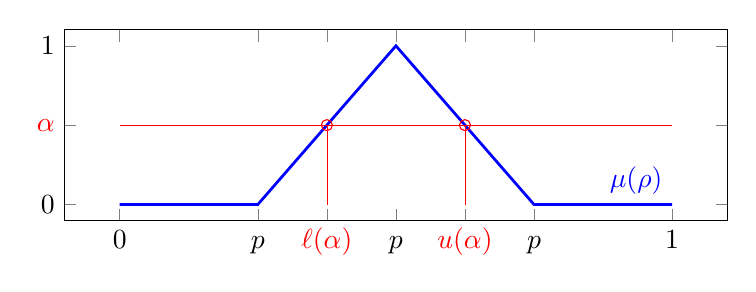
\begin{tikzpicture}
    \linespread{1}
    \begin{axis}[
        width            = 10cm,
        height           = 4cm,
        xtick            = {0, 1, 1.5, 2, 2.5, 3, 4},
        xticklabels      = {0, 
                            $\pl{p}$, 
                            \textcolor{red}{$\ell(\alpha)$}, 
                            $p$, 
                            \textcolor{red}{$u(\alpha)$}, 
                            $\pu{p}$, 
                            1},
        xticklabel style = {text height = 1.5ex},
        ytick            = {0, 0.5, 1},
        yticklabels      = {0, \textcolor{red}{$\alpha$}, 1}]

        \addplot[
            line width   = 1pt,
            mark         = none,
            draw         = blue]
            coordinates {
                (0,0)
                (1,0)
                (2,1)
                (3,0)
                (4,0)
            };
        \draw[ultra thin, red] (axis cs:0, 0.5) -- (axis cs:4, 0.5);
        \addplot[only marks, mark = o, red] coordinates {(1.5, 0.5) (2.5, 0.5)};

        \draw[ultra thin, red] (axis cs:1.5, 0.5) -- (axis cs:1.5, 0);
        \draw[ultra thin, red] (axis cs:2.5, 0.5) -- (axis cs:2.5, 0);

        \node[anchor = south east, blue] at (axis cs:4,0) {$\mu(\rho)$};
    \end{axis}
\end{tikzpicture} 